

\documentclass[
12pt,
a4paper,
pdftex,
czech,
titlepage
]{report}

\usepackage[czech]{babel}
\usepackage[utf8]{inputenc}
\usepackage{lmodern}
\usepackage{textcomp}
\usepackage[T1]{fontenc}
\usepackage{amsfonts}
\usepackage{titlesec}
\usepackage{graphicx}
\usepackage{lscape}
\usepackage{hyperref} 
\usepackage{amssymb}
\usepackage{pifont}
\newcommand{\cmark}{\ding{51}}
\newcommand{\xmark}{\ding{55}}

\titleformat{\chapter}
  {\normalfont\LARGE\bfseries}{\thechapter}{1em}{}
\titlespacing*{\chapter}{0pt}{0ex plus 1ex minus .2ex}{2.0ex plus .2ex}

\begin{document}

\begin{titlepage}
	\vspace*{-2cm}
	{\centering
\includegraphics[scale=1.0]{img/logo.pdf}\par}
	\centering
	\vspace*{2cm}
	{\Large Semestrální práce z KIV/DBM2\par}
	\vspace{1.5cm}
	{\Huge\bfseries Jednoduchá paměť na SPARQL dotazy v čistém JS\par}
	\vspace{2cm}

	{\Large Ondřej Váně, Jan Smolař\par}

	\vfill

	{\Large 3.\,12.\,2019}
\end{titlepage}

\tableofcontents
\thispagestyle{empty}
\clearpage

\begin{landscape}
	\setcounter{page}{1}
	\chapter{Celkový vzhled}
	\begin{figure}[h]
		\centering
		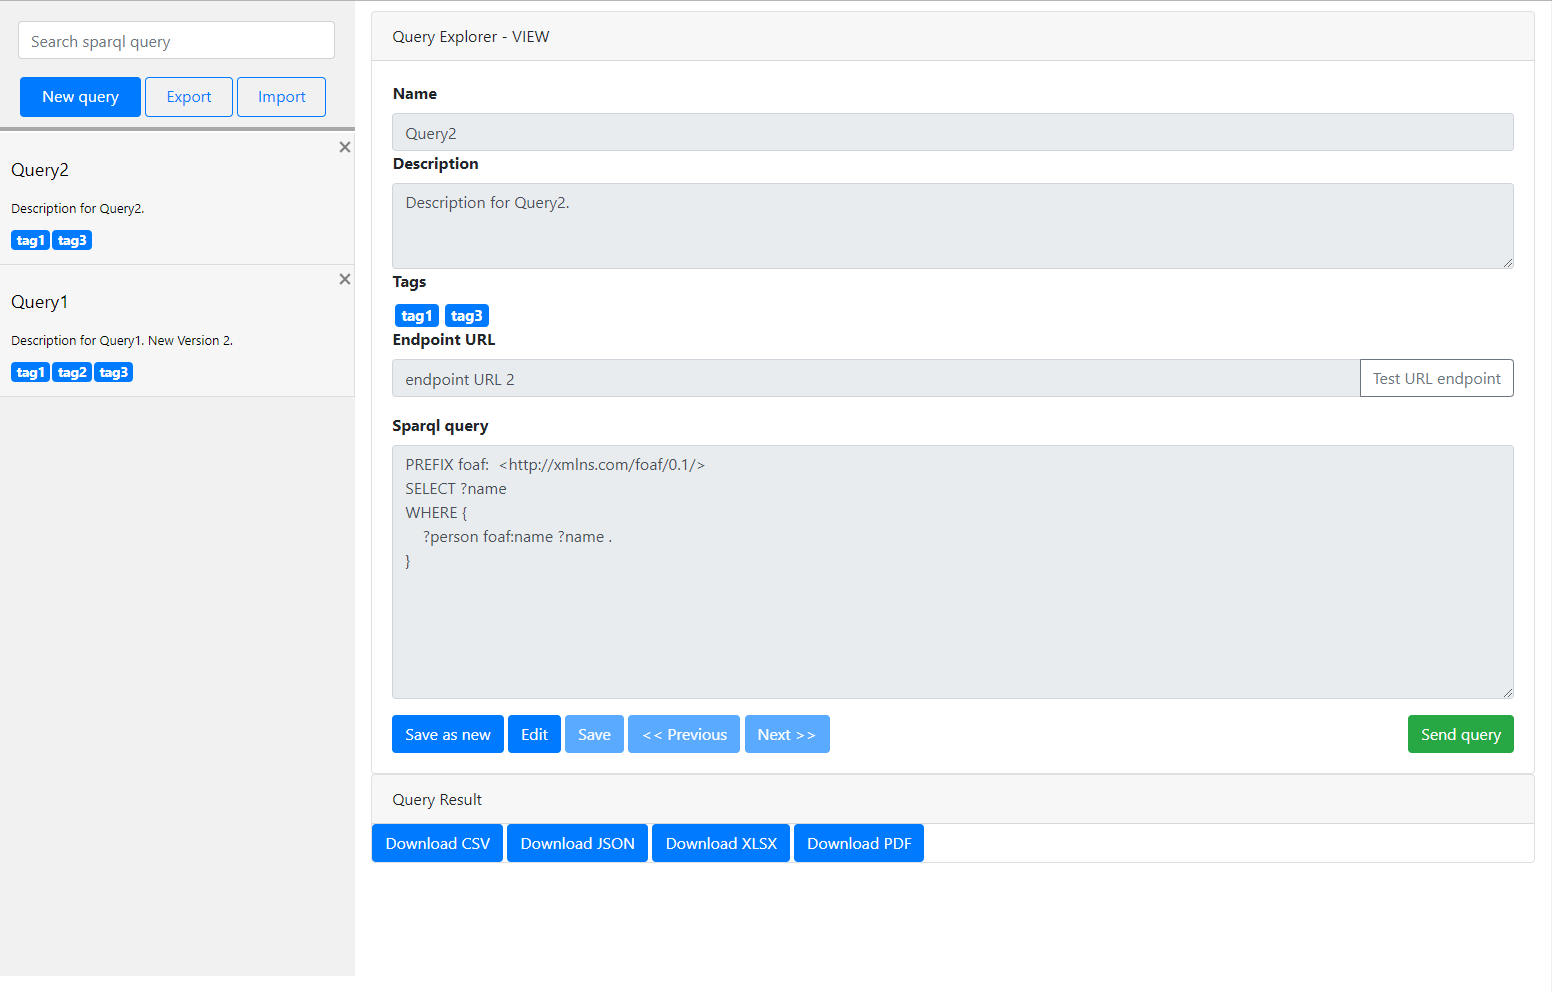
\includegraphics[scale=0.36]{img/pic1.png}
		\caption{Vzhled aplikace}
		\label{img1}
	\end{figure}
\end{landscape}



\chapter{Zadání}
Vytvořit Javascriptový nástroj, který bude snadno vložitelný do jiných webových projektů (ideálně jeden javascript soubor k načtení v html hlavičce) a bude umět:
\begin{itemize}
	\item odeslat SPARQL dotaz na zadaný libovolný SPARQL endpoint (ajax)
	\item vypsat výsledek dotazu do triviální webové tabulky
	\item exportovat výsledky dotazu
	\item načíst/uložit dotaz do místní paměti problížeče (browser local storage)
	\item spravovat uložené dotazy - mazat, aktualizovat
	\item vyhledávat v uložených dotazech
	\item exportovat/importovat dotazy
\end{itemize}

\chapter{Analýza}
K vytvoření aplikace jsme využili programovací jazyk JavaScript, jak bylo uvedeno v zadání. Pro tvorbu vzhledu stránky jsme použili framework Bootstrap a k zobrazení výsledku dotazu do tabulky framework Tabulator.io. Implemetaci aplikace jsme založili na architektuře MVC. Aplikace tedy obsahuje moduly pro komunikaci s uživatelem, pro zpracování požadavků, pro zobrazení výsledků a další.\\Hlavní překážkou bylo vytvoření struktury dotazu pro snadné a rychlé ukládání dat do lokální paměti webového prohlížeče. K ukládání dat jsme nakonec použili datový typ JSON, který obsahuje pro každý dotaz číslo poslední vytvořené verze a jednotlivé verze dotazu. Každá verze dotazu obsahuje vlastní parametry, a to jednoznačný identifikátor, popis, jméno, URL endpointu, tagy, SPARQL dotaz a číslo verze.\\Pro zobrazování výsledků dotazů nám byla navržena knihovna Sensei-grid. Po blížším prozkoumání jejích funkcí jsme došli k závěru, že pro naši práci nebude zcela optimální. Hlavními nedostatky byla neschopnost stránkování, vyhledávání a jednoduchá úprava tabulky s výsledky dotazů. Následoval tedy průzkum volně dostupných knihoven a frameworků vhodných pro naše použití. Po diskuzi jsme se usnesli na použití knihovny Tabulator.io, která poskytuje všechny potřebné funkce pro naši aplikaci.

\begin{center}
	\begin{tabular}{ | c || c | c | c | c | c | }
		\hline
		& procházení Tab & stránkování  & vyhledávání & řazení & export\\ \hline
		Sensei Grid & \cmark & \xmark &\xmark & \xmark & \xmark \\
		Tabulator & \cmark & \cmark & \cmark & \cmark & \cmark \\
		\hline
	\end{tabular}
\end{center}

\chapter{Implementace}
\section{Architektura aplikace}
Hlavním souborem celého projektu je soubor \textit{index.html}, který importuje všechny ostatní moduly, které jsou nezbytné ke správnému chodu aplikace. Dále je v souboru \textit{index.html} definováno uživatelské rozhraní celkové aplikace. Pro stylování uživatelského rozhraní byl využit framework Bootstrap a běžné kaskádové styly.
\par
Celková logika aplikace je rozdělena do jednotlivých modulů(souborů), které oddělují jednotlivé funkce, dle jejich využití. Na obrázku číslo \ref{img_arch} jsou zobrazeny hlavní moduly celé aplikace.
\begin{figure}[h]
	\centering
	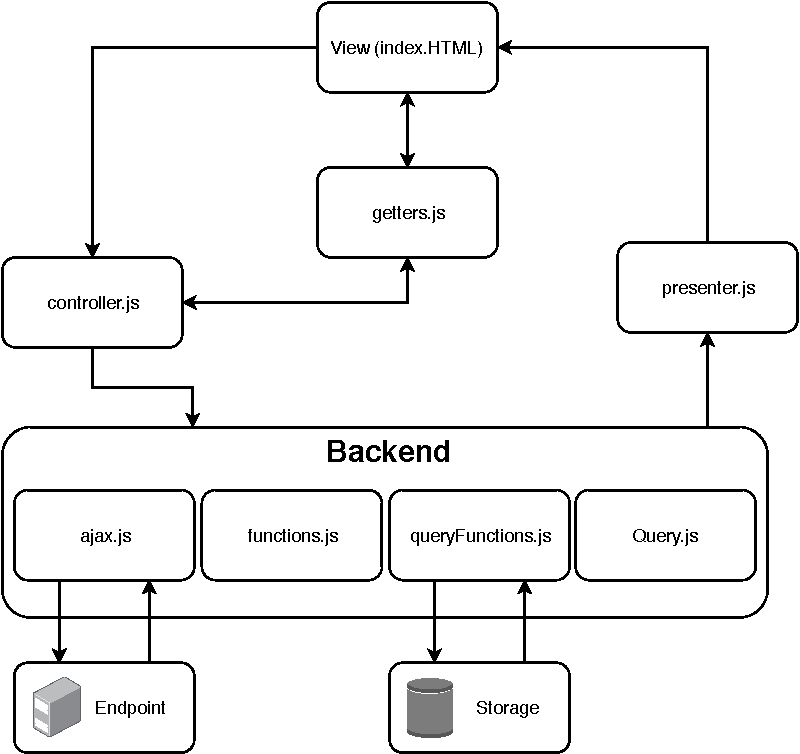
\includegraphics[scale=0.7]{img/SparqlRepositoryArchitecture.pdf}
	\caption{Architektura aplikace}
	\label{img_arch}
\end{figure}
\\
V následujícím seznamu jsou posány jednotlivé moduly a jejich funkce:
\begin{itemize}
	\item \textit{index.html} -- Hlavní soubor celého projektu, který obsahuje definici uživatelského rozhraní a importuje všechny potřebné moduly a knihovny.
	\item \textit{controller.js} -- Obsahuje metody, které jsou volané na základě uživatelské akce.
	\item \textit{presenter.js} -- Modul obsahující metody pro změnu uživatelského rozhraní na základě uživatelských akcí.
	\item \textit{getters.js} -- Obsahuje funkce pro získávání jednotlivých elementů v aplikaci.
	\item \textit{ajax.js} -- Obsahuje funkci pro asynchronní odeslání dotazu na zadaný endpoint.
	\item \textit{functions.js} -- Všeobecné funkce, které jsou používány v celém projektu.
	\item \textit{queryFunctions.js} -- Modul obsahující metody pro práci s lokálním úložištěm v prohlížeči. Ukládání, načtení a mazání dotazu z úložiště.
	\item \textit{Query.js} -- Objekt pro práci s dotazem, který obsahuje všechny potřebné údaje (id, verzi, dotaz, url endpoint, název, popis a tagy).
	\item \textit{messages.js} -- Obsahuje všechny zprávy, které jsou zobrazovány uživateli. Zprávy lze upravit do jiného jazyka.
	\item \textit{colors.js} -- Definice barev, které jsou využity v aplikaci.
	\item \textit{variables.js} -- Obsahuje globální proměnné a konstanty.
\end{itemize}
\section{Struktura aplikace}	
Struktura projektu dle adresářové struktury je zobrazena na obrázku číslo \ref{img_struc}.					
\begin{figure}[h]
	\centering
	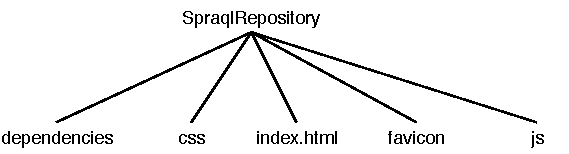
\includegraphics[scale=1.0]{img/file_tree.pdf}
	\caption{Strunktura aplikace}
	\label{img_struc}
\end{figure}
\\
V následujícím seznamu jsou popsány jednotlivé adresáře projektu:
\begin{itemize}
	\item \textit{dependencies} -- Adresář obsahující všechny knihovny, na kterých je projekt závislý.
	\item \textit{css} -- Adresář obsahující kaskádové styly.
	\item \textit{favicon} -- Adresář s ikonou, která se zobrazuje v liště prohlížeče.
	\item \textit{js} -- Adresář obsahující všechny soubory s javascriptem.
\end{itemize}
\section{Ukládání do lokálního úložiště prohlížeče}
Lokální úložiště (dále jen LÚ) umožňuje ukládat informace o relaci u klienta v podobě klíč / hodnota. Data se nepřenáší na vzdálený server a storage je funkční ve všech moderních prohlížečích. Data jsou ukládána ve fromě řetězce a LÚ neobsahuje žádnou kontrolu konzistence dat nebo generování id.
\par
Ve výsledné aplikaci je každý dotaz se všemi verzemi ukládán ve formátu JSON a jako přístupový klíč je id. Formát JSONu pro ukládání dotazu je zobrazen na obrázku číslo \ref{img_json}. Klíč id je vygenerován z globální proměnné \textit{id} (inkrementuje o jedničku), která je uložena v LÚ pro generování jednoznačného identifikátoru. Dále jsou v LÚ dvě globální proměnné s názvem \textit{currentId} a \textit{currentVersionId}. \textit{CurrentId} určuje jaký dotaz je aktuálně zobrazen uživateli a proměnná \textit{currentVersionId} je identifikátor aktuální zobrazené verze dotazu.
\begin{figure}[h]
	\centering
	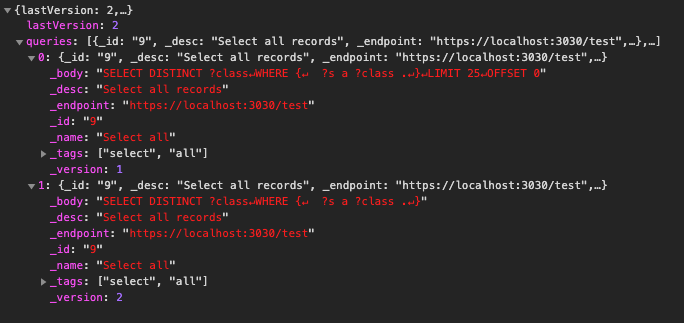
\includegraphics[scale=0.55]{img/json.png}
	\caption{Struntkrura ukládaného dotazu}
	\label{img_json}
\end{figure}
\chapter{Uživatelská příručka}
Aplikace umožňuje importovat a exportovat uložené dotazy pro přenos mezi zařízeními, vytvářet nové dotazy nebo nové verze určitého dotazu, mazat dotazy, odesílat dotazy na uvedený URL endpoint a zobrazovat jeho výsledky. Stránka je rozdělena na dvě části, a to na levý panel, který slouží pro práci s uloženými dotazy a zbytek stránky, který se používá pro úpravu a tvorbu nových dotazů.\\ \\Ovládání aplikace je zprostředkováno pomocí tlačítek na stránce:
\begin{itemize}
	\item New - vytvoření prázdné šablony pro tvorbu nového dotazu
	\item Export - uložení aktuálního stavu lokálního úložiště
	\item Import - nahrání dat do lokálního úložiště
	\item Save as new - uložení zadaných informací jako nový dotaz
	\item Edit - zapnutí/vypnutí etitačního módu
	\item Save - uložení zadaných informací jako novou verzi dotazu
	\item Previous - přepnutí na předchozí verzi dotazu
	\item Next - přepnutí na následující verzi dotazu
	\item Send query - odeslání SPARQL dotazu na zadaný URL endpoint
	\item Test URL endpoint - otestování připojení k zadanému URL endpointu
	\item Download *formát* - stažení výsledku SPARQL dotazu
\end{itemize}
\chapter{Závěr}
Vytvořená práce splňuje požadavky zadání. Při tvorbě aplikace jsme se seznámili s programovacím jazykem JavaScript. Také jsme poznali a naučili se používat lokální úložiště webových prohlížečů. Semestrální práce přispěla ke zlepšení práce v týmu jako rozdělování práce, komunikace či paralelní tvorba.
\\\\Odkaz na repozitář: \url{https://github.com/OndrejVane/SparqlRepository}
\section{Odpovědi/řešení} 
	\begin{enumerate}
		\item  \textbf{Problém:} Pokud je něco jiného [např. 2] ve web storage, váš program to zřejmě také čte a padne na exception [1]. V takovém stavu je možné vytvářet nové query, ale nejde používat uložené.
		Zároveň volba názvu klíče (int od 1) je poměrně nebezpečná. Doporučoval bych změnu alespoň na queryXXX, kde X je ten int, nebo uložit pouze jeden klíč a až ve value rozlišovat jednotlivé query.
		\\
		\textbf{Řešení:} Názvy klíčů byly přejmenovány z přirozených čísel od 1 na řetězce \textit{query\_} následované přirozeným číslem od 1, které odpovídá id dotazu. Např. \textit{query\_1}, \textit{query\_2}.
		\\
		\url{https://github.com/OndrejVane/SparqlRepository/issues/30}
		\item  \textbf{Problém:} V případě chyby query syntaxe, ale možná i jindy, se sice error vypíše do konzole, ale na samotné stránce není ani info o chybovém stavu, ani jeho popis. Bylo by dobré dodělat, klidně i jen vložením jako obyčejný text ideálně někam nad query result a pod send query button.
		\\
		\textbf{Řešení:} Pokud dojde k nějaké chybě při odesílání dotazu na endpoint, tak se chybová zpráva vypíše pod ovládací tlačítka s prefixem Error message.\\ \url{https://github.com/OndrejVane/SparqlRepository/issues/32}
		\item  \textbf{Problém:} zrušte prosím možnost editace tabulky výsledků (byl to jen experiment na ověření funkcionality knihovny). Nevíte náhodou, jestli se v tabulce jde navigovat kromě dolů/nahoru pomocí kláves "šipka nahoru/dolů" i doleva/doprava nějakým způsobem?
		\\
		\textbf{Řešení:} Editace tabulky zrušena viz issue \#31. Navigovat se po tabulce lze pouze pomocí šipek dolů/nahoru a pro horizontální navigaci lze použít klávesy TAB(do prava)/ TAB + SHIFT( do leva).
		\\
		\url{https://github.com/OndrejVane/SparqlRepository/issues/31}
		\item  \textbf{Problém:} Alespoň náznakem do dokumentace uvést, jak by bylo možné implementovat funkcionalitu na zobrazení prefixovaného URL ve výsledcích dle prefixů z dotazu. Tzn. na vstupu budu mít "prefix mreid: <http://mre.zcu.cz/id/>" a chtěl bych v tabulce místo\\ "http://mre.zcu.cz/id/12345" vidět "mreid:12345".
		\\
		\textbf{Řešení:} V nastavení přidána hodnota s názvem showShortUrl, která udává, zda se budou zobrazovat normální URI nebo zkrácené. Pokud je tato hodnota nastavena na \textit{true}, tak jde každá přijatá hodnota přes funkci s názvem \textit{parseUri}, kde je možno doimplementovat parsování uri dle potřeby.
		\\
		\url{https://github.com/OndrejVane/SparqlRepository/issues/33}
	\end{enumerate}
\end{document}